\section{BEE Framework Design}
\texttt{BEE} framework is designed to efficiently organize and manage available computing resources, automatically deploy a Docker-enabled environment, and execute a user's Dockerized application with constant monitoring and scheduling. 

As shown in \textbf{Algorithm \ref{bee}}, we outline the general workflow of \texttt{BEE} framework. First, users need to provide all the computing resources available. This can be HPC systems or cloud computing systems or both with priorities of using these computing resources. For example, when running a compute intensive application, users may want to prioritize systems with higher computing performance. Then, users need to provide a Dockerized application with an input stack and a configuration file.

Before execution, \texttt{BEE} picks the system with the highest priority (\textbf{Line 3}). Then, it deploys the Docker-enabled execution environment on the target system. If the execution target environment is HPC system, \texttt{BEE-VM} is deployed. If the execution target environment is AWS or Chameleon Clound, then \texttt{BEE-AWS} or \texttt{BEE-Chameleon} is applied. Both will be discussed in later sections. After the execution environment is deployed, BEE checks whether the current application is in an initial stage or needs to restore from a previous checkpoint. If it is in an initial stage, \texttt{BEE} attaches the input stack and runs the application as shown in \textbf{Line 8 and 10}. Otherwise, \texttt{BEE} first migrates previous intermediate data checkpoints from the previous system to the current system (\textbf{Line 5}) then attaches the data and restores the checkpoint (\textbf{Line 6}) before running. 

During execution, \texttt{BEE} monitors the current state of the running application. When it is close to the end of the current time slot, \texttt{BEE} checks whether the current application has completed. If so, \texttt{BEE} outputs the result and stops. Otherwise, if the application has a checkpointing procedure and is indicated by the user, \texttt{BEE} initiates the checkpointing procedure and marks $need\_migration$ to ensure the application will resume from the current execution stage for later runs. When finishing the checkpointing procedure, \texttt{BEE} checks for the next available system to run. If no other computing systems are available, \texttt{BEE} saves the checkpoint to disk, until the user indicates new computing resources are available.
	

\begin{algorithm}
\caption{BEE Framework}
\label{bee}
\begin{algorithmic}[1]
\REQUIRE{$HPC/Cloud_1$: [Host node: $H_1$, $H_2$,..., $H_k$][Time slot: $T_1$]}
\REQUIRE{$HPC/Cloud_2$: [Host node: $H_1$, $H_2$,..., $H_k$][Time slot: $T_2$]}

{...}

\REQUIRE{$HPC/Cloud_m$: [Host node: $H_1$, $H_2$,..., $H_k$][Time slot: $T_m$]}
\REQUIRE{Computing resource priority list: $L$}
\REQUIRE{User Dockerized application}
\REQUIRE{Input data: $D$}
\REQUIRE{User defined hardware configuration: uconf}

\STATE $need\_migration \leftarrow$ False
\STATE $lastHost \leftarrow$ N/A

\WHILE{H $\leftarrow$ get\_top($L$)}
	\IF{$need\_migration$ is True}
		\STATE data\_tranfer($lastHost$, $H$, $D$)
		\STATE restore\_data\_checkpoint($D$, $H$) \bluecomment{Load data checkpoint into H}
	\ELSE
		\STATE load\_initial\_data($D$, $H$) \bluecomment{Load initial data into H}
	\ENDIF
	
	\bluecomment{Deploy BEE-VM or BEE-AWS}
	
	\STATE deploy\_bee($H$, $user\_application$, $uconf$)

	\WHILE{$H$ running normal AND Running-time not close to $T$}
		\STATE Monitor($H$)
	\ENDWHILE

	\IF{execution incomplete}
    	\STATE pause($H$)
		\STATE $D \leftarrow$ data\_checkpoint($H$) \bluecomment{Checkpoint application data}
		\STATE $need\_migration \leftarrow$ True
		\STATE $lastHost \leftarrow$ H
		\STATE stop($H$)
	\ELSE
		\STATE stop($H$)
		\STATE result $\leftarrow D $
		\STATE terminate() 
	\ENDIF
\ENDWHILE

\IF{execution incomplete}
		\STATE $D\leftarrow$ data\_checkpoint($H$)
		\STATE stop($H$)
		\STATE store $D$ when no resource available
\ENDIF

\end{algorithmic}
\end{algorithm}


\section{BEE-VM Design}
Linux container technologies (e.g., Docker) enable consistent software and hardware environments for development, build, and deployment. By using Docker, developers only need to build their application once in a Docker container image on their local machine; then, the dockerized application can run on any Docker-enabled machine. However, Docker is not supported on production HPC systems. Existing containerization solutions on current HPC systems typically require customized HPC environments. The lack of a robust and universal solution to containerization in HPC and the requirement of system customization limits the practicality of container deployments across HPC machines.
  
To overcome the constraints and provide a more flexible runtime environment, we designed a backend for \texttt{BEE}, the \texttt{BEE-VM}, which creates a VM layer on top of the host and then deploys Docker on the VM layer; as shown in \textbf{Fig. \ref{bee-framework}}. Besides providing a standard updated Docker capability to HPC system, additionally the VM layer also brings the following advantages: First, with full control over VM, we can create consistent environments for Docker across platforms. As a result, we can deploy \texttt{BEE} on both HPC and AWS with user applications unmodified. Second, Docker containerization ensures the reproducibility across  different software stacks and OSes, while VM guarantees the reproducibility accross different hardware infrastructures, which can be a problem if the container is running directly on the host.  

\begin{figure}[h]
%\vspace*{-1em}
    \centering
    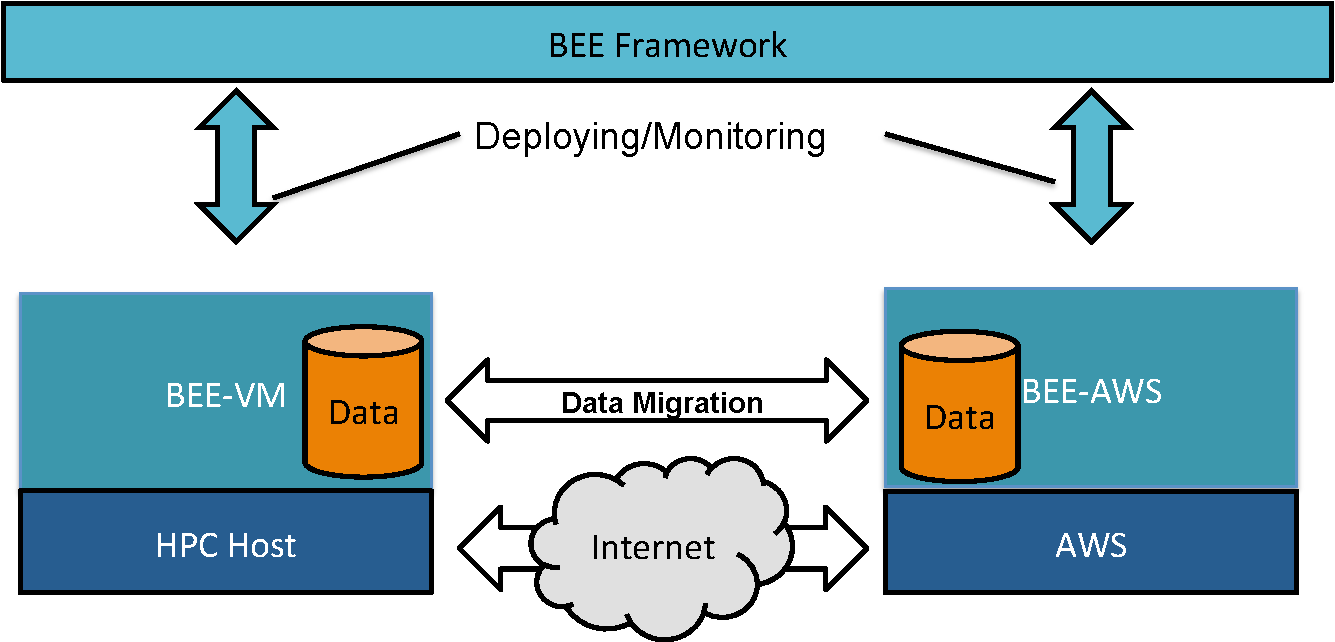
\includegraphics[width=0.35\textwidth]{figures/bee-framework.pdf}
    \caption{BEE Framework}
    \label{bee-framework}
%\vspace*{-1em}
\end{figure}


 The design details of \texttt{BEE-VM} include several parts: network design, storage design, and BEE-VM deployment process. We discuss them in detail in the following sections.
 
\subsection{Network Design}
The network design of \texttt{BEE-VM} mainly targets two functions. First, we need to dynamically configure and deploy our VM and Docker container. This needs to be done automatically and remotely by \texttt{BEE}. We choose to utilize SSH for remote configuration. Also, since we are aiming at HPC application and most HPC applications require MPI, we need to dynamically compose a network for MPI communication between different computing nodes. For enabling that, we create a virtual subnet comprised of all VMs and corresponding Docker containers, so that they can communicate with each other.

\subsubsection{VM layer}
We first discuss the network design at the VM layer. This is necessary because the Docker container will rely on the VM's network configuration for network in the container. 

In order to enable the SSH connection to the VM through the host, the hypervisor is configured to use port forwarding to map an unused port on the host to the SSH port on the VM. However, this makes the virtual network interface card (vNIC) hard to utilize by MPI. Although some MPI libraries can be configured to use a designated port and can cooperate with port forwarding, many commonly used MPI libraries (e.g., OpenMPI) use random ports, which is not easy to work with the port forwarding mechanism. So, we created a second vNIC dedicated for MPI communication. 

However, allowing application in different node communication to each other through the second vNIC is challenging. The main challenges of designing the network for VMs is that the root privileges are not assigned to regular user but most of the suitable VM networking configurations do require root privileges (e.g., bridging network). To address this limitation, we designed two user space solutions for connecting all second vNICs on HPC systems.



\begin{comment}
\textbf{Solution 1: 2 NICs}
We design our first solution on the `Galton` nodes of our testbed cluster machine. Each `Galton` node has two physical NICs. So, we use the port forwarding combining the SSH virtual NIC with one physical NIC and use simple pass-through mode to combine the MPI virtual NIC with the other physical NIC. This is the simplest design in our two solutions. However, this solution is limited to deployment on computing nodes with multiple physical NICs. 

\begin{figure}[h]
    \centering
    \caption{Network Design using two NICs}
    \label{2nic}
    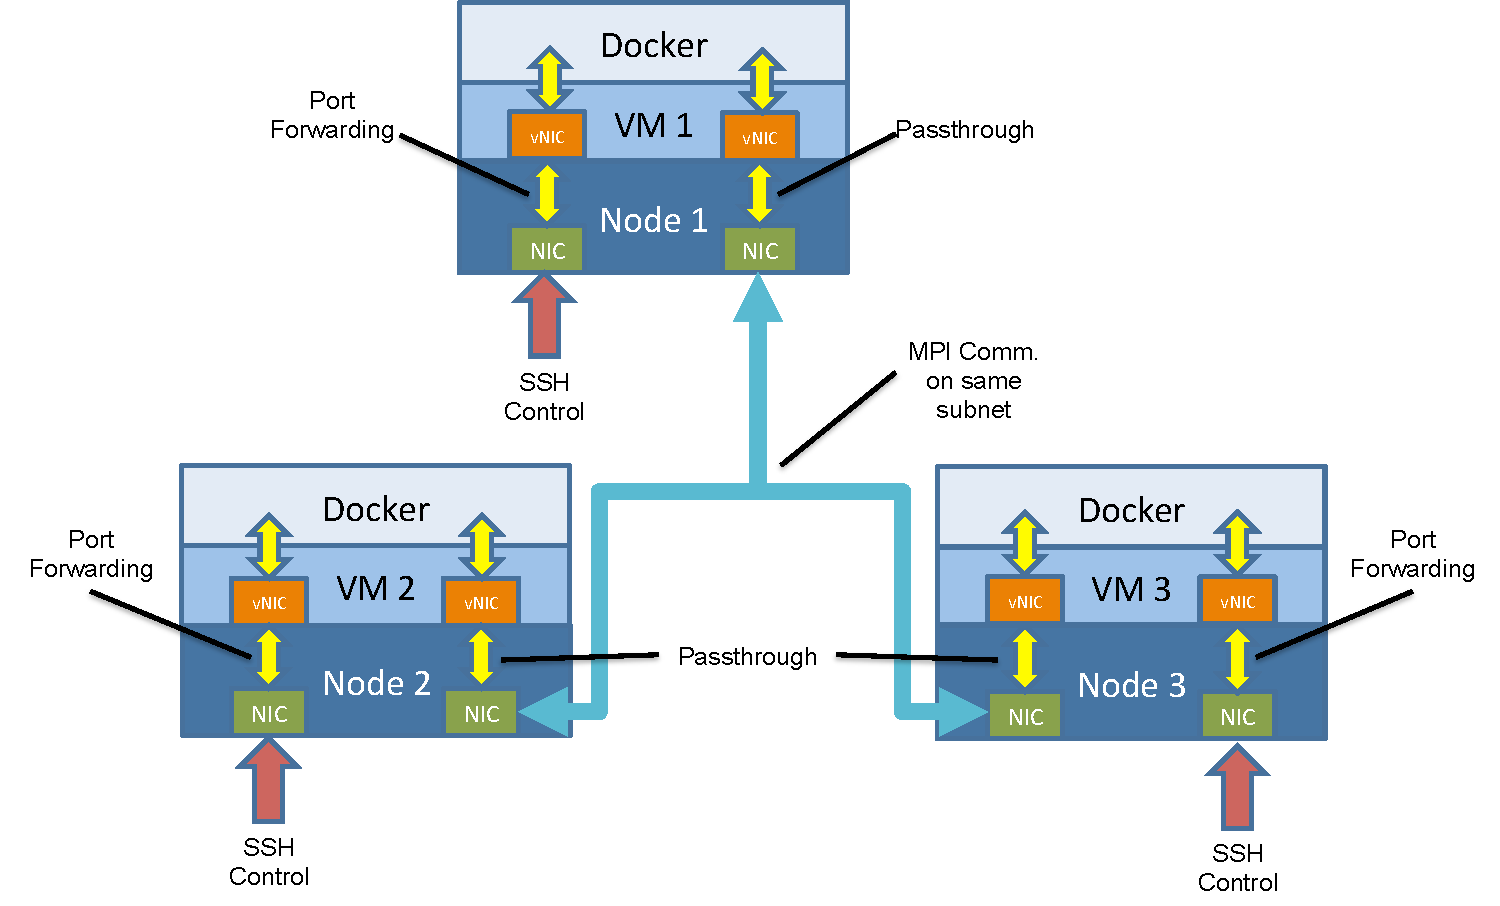
\includegraphics[width=0.5\textwidth]{figures/2nic.pdf}
\end{figure}

\end{comment}
 
\textbf{Network Solution 1: Multi-cast}
In the first solution, we use multi-cast subnet to connect all second vNICs of all VMs together for MPI communication. Since all vNICs are connected to the same subnet, there is no restriction on port usage, so any MPI library can be used. The advantage of this design is that the configuration is simple, and if one node in the multi-cast network failed, it will not affect the connection in between other nodes, which can easily cooperate with a potential fault tolerance mechanism. This network design works best on applications with intensive all-to-all or one-to-all communications, since all packages are naturally sent to all nodes. However, if one-to-one communication is more frequent, the multi-cast network brings high communication overhead, since it generates more data packages in the subnet than necessary. 

\begin{figure}[h]
	%\vspace*{-1em}
    \centering
    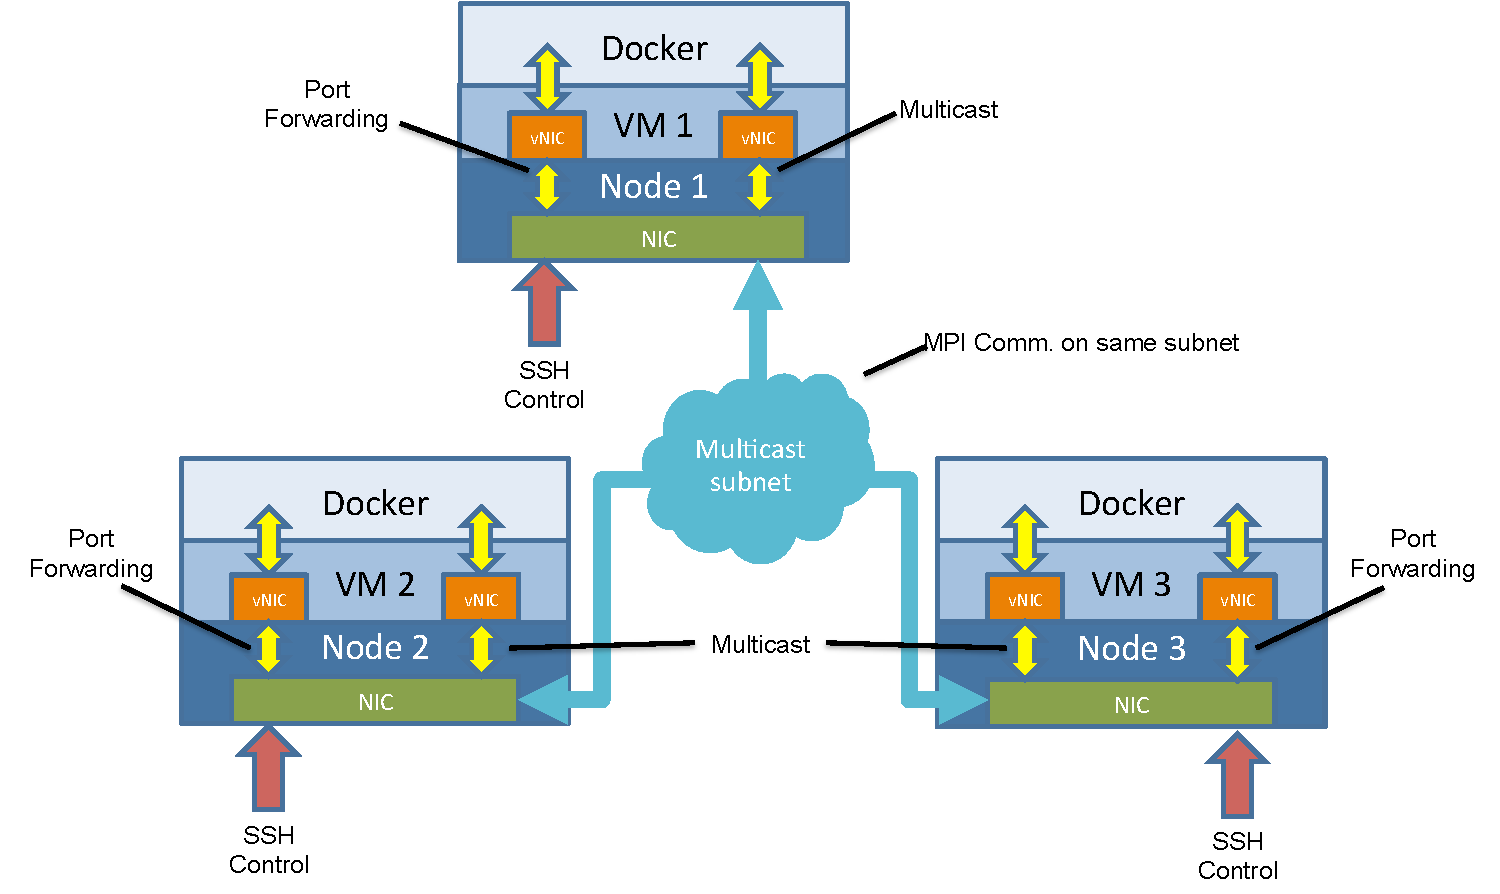
\includegraphics[width=0.5\textwidth]{figures/mcast.pdf}
    \caption{Network Design using Multi-cast}
    \label{mcast}
    %\vspace*{-1em}
\end{figure}

 
\textbf{Network Solution 2: P2P sockets}
In our second solution, we connect each second vNIC from each VM using point-to-point (P2P) socket connection. This is similar to the wired Ethernet connection between computing nodes in HPC system, except instead of relying on a physical switch we map out a specific routing topology. Since there is a P2P routing path between nodes, there are no unnecessary data packages in the network. However, socket connections between nodes may route via intermediate nodes, so if one node fails, it may break several connected nodes, complicating any potential fault tolerance mechanisms. Also, the performance of this kind of network is affected by the connection pattern between nodes, so we adopt two connection patterns in this solution (more patterns will be studied in the future).

\begin{figure}[h]
  	%\vspace*{-1em}
    \centering
    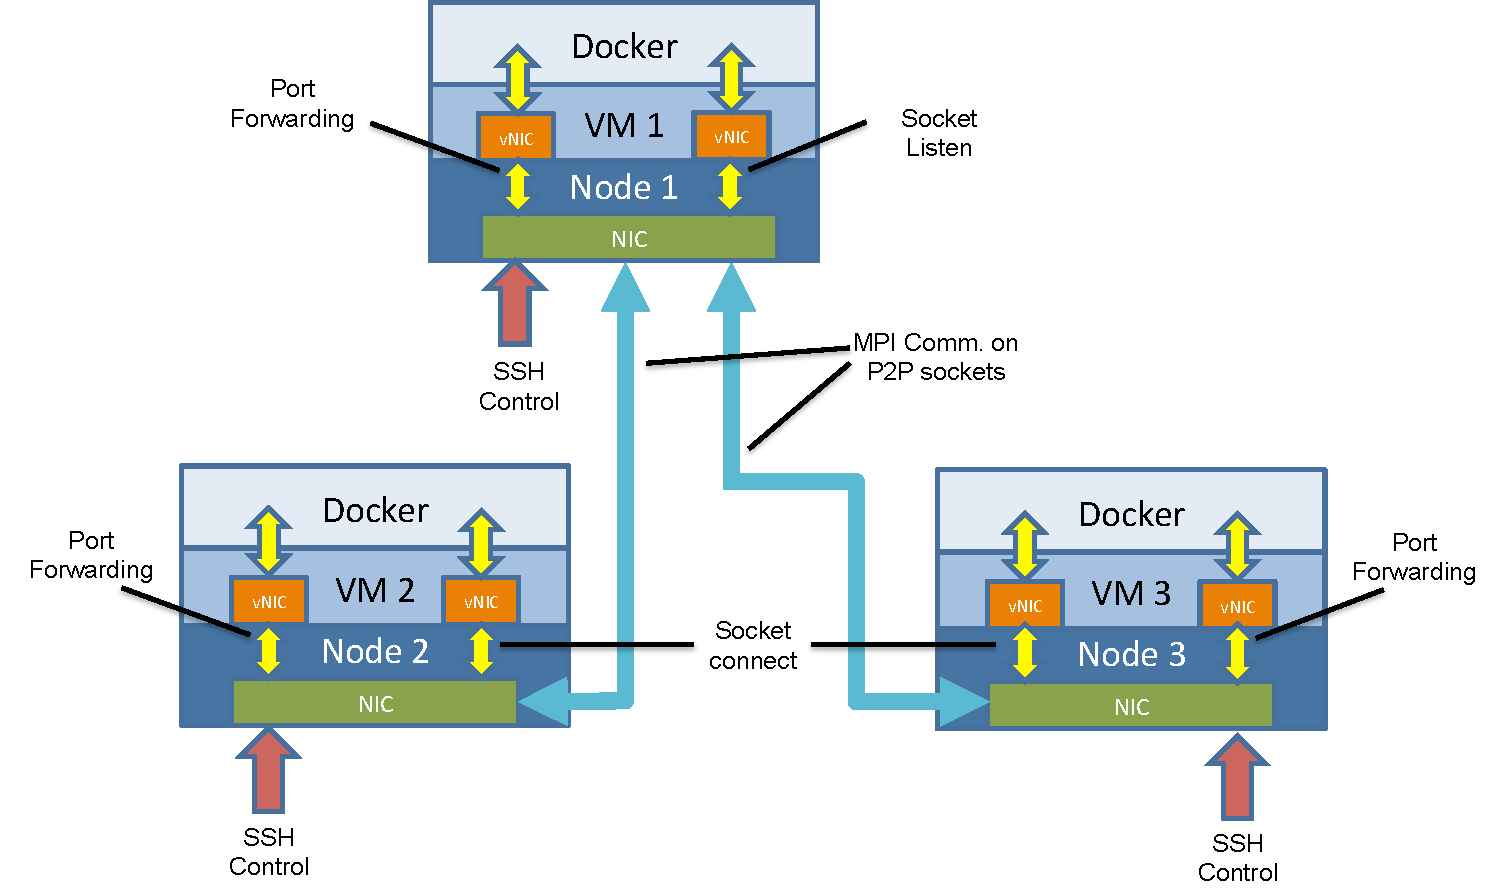
\includegraphics[width=0.5\textwidth]{figures/p2p.pdf}
    \caption{Network Design using P2P sockets}
    \label{p2p}
    %\vspace*{-1em}
\end{figure}

\begin{itemize}
\item \textbf{Star-shaped connection}
In the first approach, we connect nodes using star-shaped topology with the master node in the center. This connection pattern can effectively minimize connection hops between each pair of nodes ($O(1)$). However, since all communication must go through the center node, it may become a hot stop in the network, especially for applications involve intensive network communication or the shared storage design that requires network communication.
\item \textbf{Tree-shaped connection}
The second way to connect all nodes is using tree-shaped topology with the master node as the tree root. In this design, we use a binary tree structure. This connection can mitigate the hot spot issue, but it also increases connection hops between each pair of nodes ($O(n\log{n})$). 
\end{itemize}

\subsubsection{Docker container layer}
Based on the network of VM layer, we design the network between Docker containers. There are several network configurations for the Docker containers; however, to minimize network overhead, the most direct configuration is network pass-through. Essentially, all network interfaces on the VM are exposed to the Docker container. Since there is no additional buffer or translation in between, it brings the least overhead. However, it is also considered as the least secure configuration, since everything is exposed. But since we deploy the Docker inside VM, this extra layer already provides enough isolation, so there is no extra security issue here. Since the presented network interfaces are exactly the same between the VM and the Docker container inside it, the software level configuration (e.g., SSH, MPI, etc.) is exactly the same.

\subsection{Storage Design}
\subsubsection{VM layer}
In this section, we discuss the design of shared storage system of \texttt{BEE-VM}. General HPC applications usually use some kind of shared file system (e.g., NFS) to share data between processes in real-time. To provide the same environment, we need to build a shared file system across different nodes in \texttt{BEE-VM}. To enable light-weight cross-platform migration, we aim to separate data from the virtualized operating system itself. This separation allows users to easily migrate their data to another platform without transferring heavy operating system files. We design two architectures to allow different processes in different nodes to share files in real-time.

\textbf{Storage Solution 1: Extra Data Image + NFS}
In our first solution, we build an extra data image and mount it as the second disk. Due to the copy-on-write characteristic of most virtual images, files updated by one machine are not visible by other machines in real-time. So, we choose to mount this data image only to the master node, and use NFS to share this mounted data disk with other VMs. By using the extra data image, data can be easily migrated.  Before computation, input data can be first loaded into the image offline. After execution, the output data is also stored in this image. To move the data to other parts of the user workflow, the user only needs to unmount the data image from the master node of the current \texttt{BEE} cluster and mount it to the master node used for the next stage computation. Also, the image encapsulation can protect data integrity. However, the data image is shared with other worker nodes via NFS, which highly depends on the performance of the virtual network. If the user's application is storage I/O intensive and the network bandwidth is limited, it may consume too much of the network resource, which may degrade MPI communication performance.


\begin{figure}[h]
	%\vspace*{-1em}
    \centering
    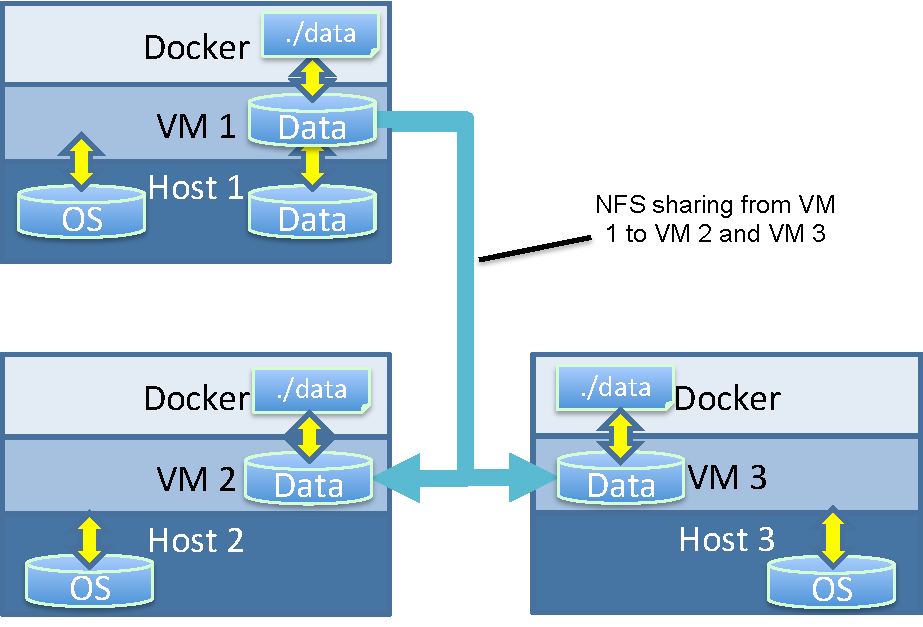
\includegraphics[width=0.5\textwidth]{figures/fs1.pdf}
    \caption{Shared Storage Design using Extra Data Image + NFS}
    \label{fs1}
\end{figure}


\begin{comment}
\subsubsection{Only NFS}
In our second solution, we aim to reduce the dependency on a virtual shared filesystem. Instead of building our own NFS sharing environment, we mount the NFS standard filesystem that is commonly used on most HPC systems. Each VM explicitly mounts the same path within the shared filesystem. Data in the same directory is shared between different host nodes via  existing fast dedicated shared hardware resources. Since a host directory is mounted, the data is also accessible from the host during execution, which can be useful for output monitoring or sampling for in-situ analysis. This is not possible if we use the first solution, since data is not readily accessible outside the data image. This solution only relies on the network between host and VM, which saves most virtual network bandwidth for MPI communication.


\begin{figure}[h]
    \centering
    \caption{Shared Storage Design using Only NFS}
    \label{fs2}
    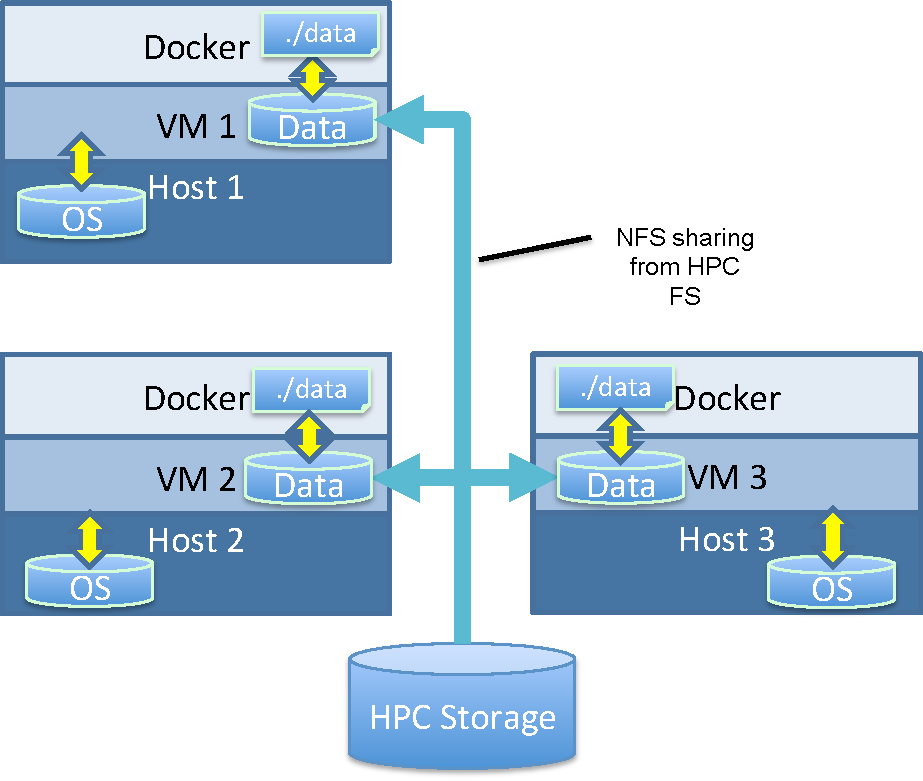
\includegraphics[width=0.4\textwidth]{figures/fs2.pdf}
\end{figure}
\end{comment}

\textbf{Storage Solution 2: Virtio}
In our second solution, we eliminate all the dependency on the virtual network. We use the Virtio feature \cite{russell2008virtio} in QEMU to map a host directory to a directory in VMs. It only requires minimum configuration at VM boot time. Each machine maps the same directory, so the data is shared using file-sharing capability that is commonly used in most HPC systems (e.g., NFS, Lustre, etc.), and it is also visible to the host in real-time. Since it does not rely on the virtual network, the whole virtual network is saved for MPI.

\begin{figure}[h]
	%\vspace*{-1em}
    \centering
    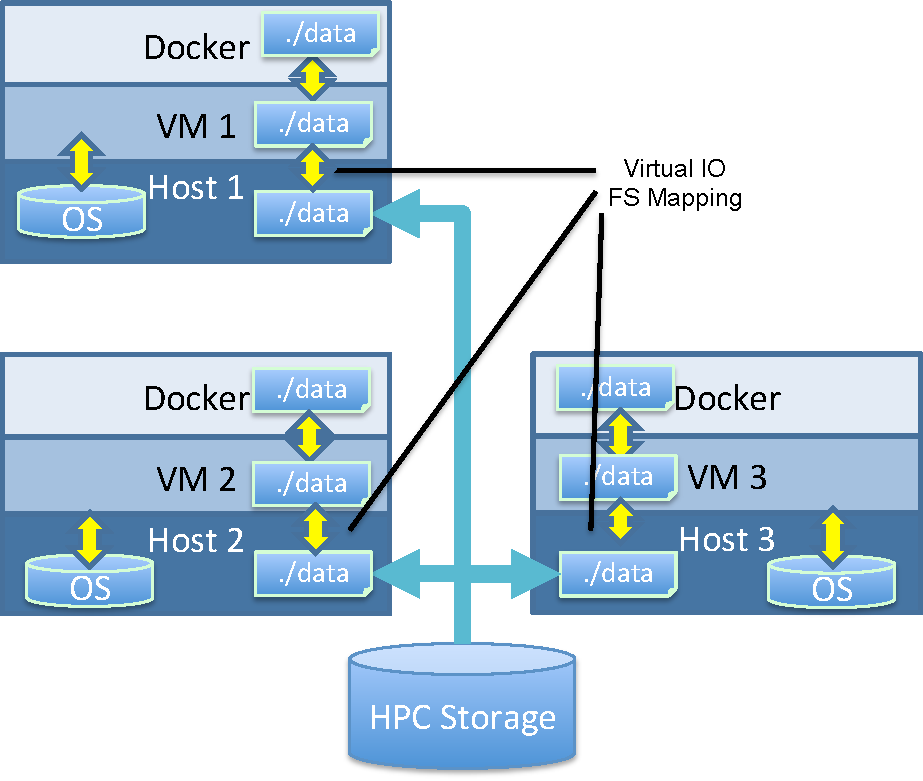
\includegraphics[width=0.5\textwidth]{figures/fs3.pdf}
    \caption{Shared Storage Design using Virtual IO}
    \label{fs3}
    %\vspace*{-1em}
\end{figure}

\subsubsection{Docker container layer}
Finally, for data sharing in the Docker layer, we use the data volume mount feature in Docker to mount the shared folder in the VM to a directory in Docker. Since Docker runs as a process at the VM layer, mounting the data volume adds negligible overhead. This configuration is also compatible with all data-shared mechanisms in the VM layer.

%\begin{comment}
\subsection{BEE-VM Builder}
VM plays an important role in \texttt{BEE-VM}. The VM is the core of \texttt{BEE-VM} that brings computing resources from host, virtual network, shared storage, user provided Dockerized application and Docker container management together. The VM in \texttt{BEE-VM} first need to be build and customized by \texttt{BEE-VM Builder} before it can be used. There are two phases in the building process:

\subsubsection{Phase 1}
The first stage in building the VM images for  \texttt{BEE-VM}. This step is done off-line before it is deployed on targeting HPC system. For uniform standard image building process, we designed our \texttt{BEE-VM Image Builder} using Packer \cite{packer}. Packer allows us to build customized images automatically. We can also run our own configure scripts in the VM image to enable more flexible customization. Although it is also possible to configure and customize VM OS in phase 2 after booting VMs, the static customization and configuration of images off-line can save a lot of time. For example, building and installing packages. We aim to minimize on-line configuration as much as possible to reduce \texttt{BEE-VM} deployment time and put most of the customization into the \texttt{BEE-VM Image Builder}. The main customization responsibilities of \texttt{BEE-VM Image Builder} include:
\begin{enumerate}
\item \textbf{Create and configure user accounts:} We need to create a user for the host to login or control the VM.
\item \textbf{Configure network interfaces:} Network interface must be configured in advance before \texttt{BEE} can configure and control the VM after it has started. However many network configurations cannot be determined until boot time, so we design a customize script built in to the image, so that network interface can be customized automatically when the VM started.
\item \textbf{Configure SSH server/client:} SSH is required for \texttt{BEE} to control VM and it is also important for MPI. So, we need to configure SSH key pairs and customized port numbers in this step.
\item \textbf{Install essential packages and tools:} Many packages and tools are required including MPI and Docker.
\item \textbf{Configure proxy settings:} Most institutional HPC system requires some kind of proxy setting in order to connect to the Internet. 
\item \textbf{Configure shared storage:} We need to pre-configure the VM image for mounting shared storage system. For example, configuring NFS server.
\end{enumerate} 

\subsubsection{Phase 2}
This phase is done when deploying \texttt{BEE-VM} on target HPC system. The base image created from phase 1 is highly reusable. Each \texttt{BEE-VM} uses the base image to create a dedicated image for the current \texttt{BEE-VM}. When \texttt{BEE-VM} started, user's Dockerized application is placed in it. This can be done in several ways. User can provide Docker image from public or private DockerHub or build Docker image from Dockerfile. After than, the building process of \texttt{BEE-VM} is done.

%\end{comment}

\subsection{BEE-VM Deployment}
\textbf{Algorithm \ref{bee-launch}} shows the workflow in \texttt{BEE} used for launching \texttt{BEE} cluster on a given platform. Although the specific process varies from HPC system to cloud computing system, the general procedures are the same. At first, the launcher needs to know how many and which nodes are available. Then, the user Dockerized application is provided, which can be in either Docker image form or Dockerfile form. Finally, a user-defined hardware configuration file may also be provided, which is used when starting VMs. 

There are four stages for launching HPC applications in \texttt{BEE}. In the first stage, a new \texttt{BEE} cluster is initialized with optional given name. This stage registers each available host to the virtual cluster. Second, \texttt{BEE-VM} deploys the VM layer. It creates one VM for each host, and then configures and assigns the VM to the  host. In \textbf{line 13}, \texttt{BEE-VM} starts a VM in parallel using MPI. In the third stage, \texttt{BEE-VM} starts to deploy the Docker layer. Depending on what the user provides, \texttt{BEE-VM} will either pull the Docker image from public/private registries or build a new Docker image from a Dockerfile loaded into the local VM. Finally, in the forth stage, \texttt{BEE} starts the application by launching from the first node (i.e., master node).


\begin{algorithm}
\caption{Deploying BEE cluster on HPC/cloud}
\label{bee-launch}
\begin{algorithmic}[1]
\REQUIRE{Allocated host nodes: $H_1$, $H_2$,..., $H_k$}
\REQUIRE{User Dockerized application (Docker image/Dockerfile)}
\REQUIRE{BEE cluster name: cname}
\REQUIRE{User defined hardware configuration: uconf}
%\STATE \textbf{[Create a new \texttt{BEE} cluster]}

\bluecomment{Create a new \texttt{BEE} cluster}
\STATE $BCluster \leftarrow$ create\_bee\_cluster(cname)
\FOR{$j=1$ to $k$}
	\STATE $BCluster$.register\_host($H_j$)
\ENDFOR
%\STATE \textbf{[Deploy VM layer]}

\bluecomment{Deploy VM layer}
\FOR{$j=1$ to $k$}
	\STATE $vm_j$ $\leftarrow$ create\_vm()
	\STATE $vm_j$.create\_img() \bluecomment{Create image for each VM}
	\STATE $vm_j$.configure(uconf) 
	\STATE $vm_j$.setup\_shared\_vol()
	\STATE $vm_j$.setup\_network()
	\STATE $H_j$.register\_vm($vm_j$)
\ENDFOR
\STATE $BCluster$.mpi\_start\_vms()
%\STATE \textbf{[Deploy Docker layer]}

\bluecomment{Deploy Docker layer}
\FOR{$j=1$ to $k$}
	\STATE $dkr_j$ $\leftarrow$ create\_doocker()
	\IF{user provides Docker image}
		\STATE $dkr_j$.img\_pull(d\_img)
	\ELSE
		\STATE $dkr_j$.img\_build(d\_file)
    \ENDIF
	$vm_j$.register\_docker($dkr_j$)
\ENDFOR
\STATE $BCluster$.mpi\_start\_dockers()
\STATE \textbf{[Start user application]}
\STATE $BCluster$.$vm_i$.$dkr_1$.start()

\end{algorithmic}
\end{algorithm}

\begin{comment}
\subsection{BEE-VM Object-oriented Design}

\begin{figure}[h]
\vspace*{-1em}
    \centering
    \caption{BEE Object-Oriented Design}
    \label{ood}
    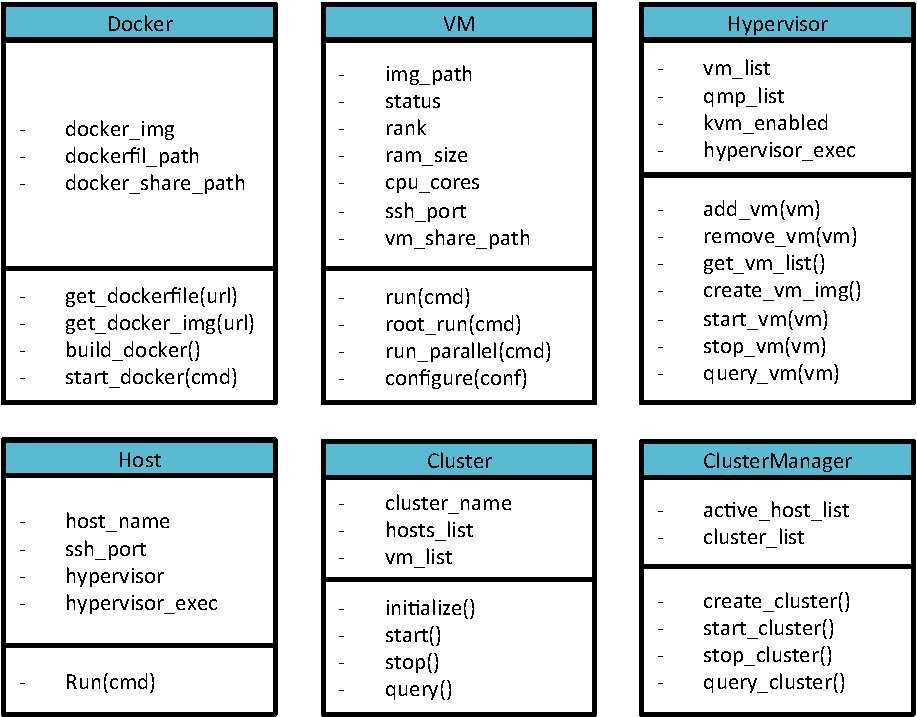
\includegraphics[width=0.5\textwidth]{figures/ood.pdf}
    \vspace*{-1em}
\end{figure}
In this section, we discuss the design details of our \texttt{BEE} framework. To better manage large scale \texttt{BEE} clusters and for extensibility consideration, we choose to use object-oriented design in python for \texttt{BEE} as shown in \textbf{Figure \ref{ood}}. We design several key classes for key components in \texttt{BEE} and \texttt{BEE-VM}, including: \texttt{Docker}, \texttt{VM}, \texttt{Hypervisor}, \texttt{Host}, \texttt{Cluster}, and \texttt{ClusterManager}. \texttt{Docker} class stores Docker-related information. For example, Docker image name, Dockerfile path, Docker's running state and the directory in Docker that is shared between containers. It also contains necessary functions to control or run commands in the Docker containers. \texttt{VM} class stores VM-related information, including the VM instance, current hardware configurations, network settings, VM image file path, shared storage directory, etc. It also has necessary functions to control the VM. However, we leave start/stop/query function to the \texttt{Hypervisor} class, since implementation of those functions are hypervisor-specific. \texttt{Hypervisor} class stores hypervisor-related information. For example, the path to the hypervisor binary, KVM availability, and a list of VMs that it are currently running. Since we allow different machine to use different hypervisors, we inherit the \texttt{Hypervisor} class to get the hypervisor class for specific hypervisors. For example, we have a \texttt{QEMU} class that is targeting for QEMU hypervisor. Besides all the functions inherited from \texttt{Hypervisor} class, it also has some QEMU-specific functions, like QMP VM monitor functions. \texttt{Host} class maintains all the information of each host, including the host name, username, port number and the hypervisor that is currently running on it. It also has functions used to execute commands on the host. \texttt{Cluster} class maintains the information of a virtual \texttt{BEE} cluster, including cluster name, all host nodes and the VMs involved, network configuration for this cluster, etc. It also has functions to control and query the cluster. \texttt{ClusterManager} class is used to manage multiple clusters on a computing system. It maintains all the active host nodes on the current system, so that they can be shared between clusters. It provides necessary functions to control each clusters. 
\end{comment}
\section{BEE-AWS Design}
AWS is a highly usable computing environment for cloud and HPC users. To provide a similar Docker-enabled environment on AWS, we designed another back-end \texttt{BEE}, the \texttt{BEE-AWS}. It enables the user to run their Dockerized application on AWS using \texttt{BEE-AWS} the same way as they run on the HPC system using \texttt{BEE-VM}. Since both the storage and network on AWS are highly optimized and their configurations are hidden from users, the design of \texttt{BEE-AWS} is relatively simpler than \texttt{BEE-VM}. In \texttt{BEE-AWS}, it first launches an AWS instance based cluster using BOTO API \cite{BOTOAPI} with optimized network configuration and a shared EFS storage. Then, it loads the user application's input data into EFS for storage sharing. Next, \texttt{BEE-AWS} controls each instance to obtain Docker images either from public/private docker registries or builds Docker images from Dockerfiles. Finally, it starts the user application in Docker containers.
\section{BEE-Chameleon}
Chameleon Cloud \cite{chameleon} is a highly configurable experimental environment for large-scale HPC and cloud research. We also designed a \texttt{BEE} backend, \texttt{BEE-Chameleon}, for delivering same Docker-enabled environment on Chameleon Cloud. So, BEE users can also run their Dockerized application on Chameleon Could without modification. Chameleon Cloud is managed by OpenStack, which allows us to launch, configure, and control instances on Chameleon Cloud through remote APIs. Chameleon Cloud enables user to have root privileges on their bare-metal machines, so we deploy the Docker layer directly on the host without the VM layer in between. Taking advantage of the Infiniband support in SR-IOV enabled instances, we also enable Infiniband support in \texttt{BEE} through a customized Infiniband-enabled \texttt{BEE} Docker base image. So, users of \texttt{BEE} can have an option to utilize accelerated network in \texttt{BEE-Chameleon} by rebuilding their Dockerized application with our new Infiniband-supported base image.